\subsection{Paired-End Reads}
Le paired-end reads consistono nell'estrazione di due letture da un singolo frammento di DNA (generalmente le due estremità), contrariamente alle single-end reads che ne estraggono solo una. Sono prodotte da sistemi NGS, e la loro preparazione è molto semplice: una volta stabilita la grandezza della singola lettura, viene estratta la lettura sull'estremità sinistra, il campione viene girato, e viene estratta nuovamente l'estremità sinistra (ottenendo quindi l'estremità destra); viene inoltre fornita la distanza tra le due letture.

%RNA-Seq?
Più nello specifico, le read utilizzate da ASGAL sono RNA-Seq.

\begin{figure}[h!]
	\centering
	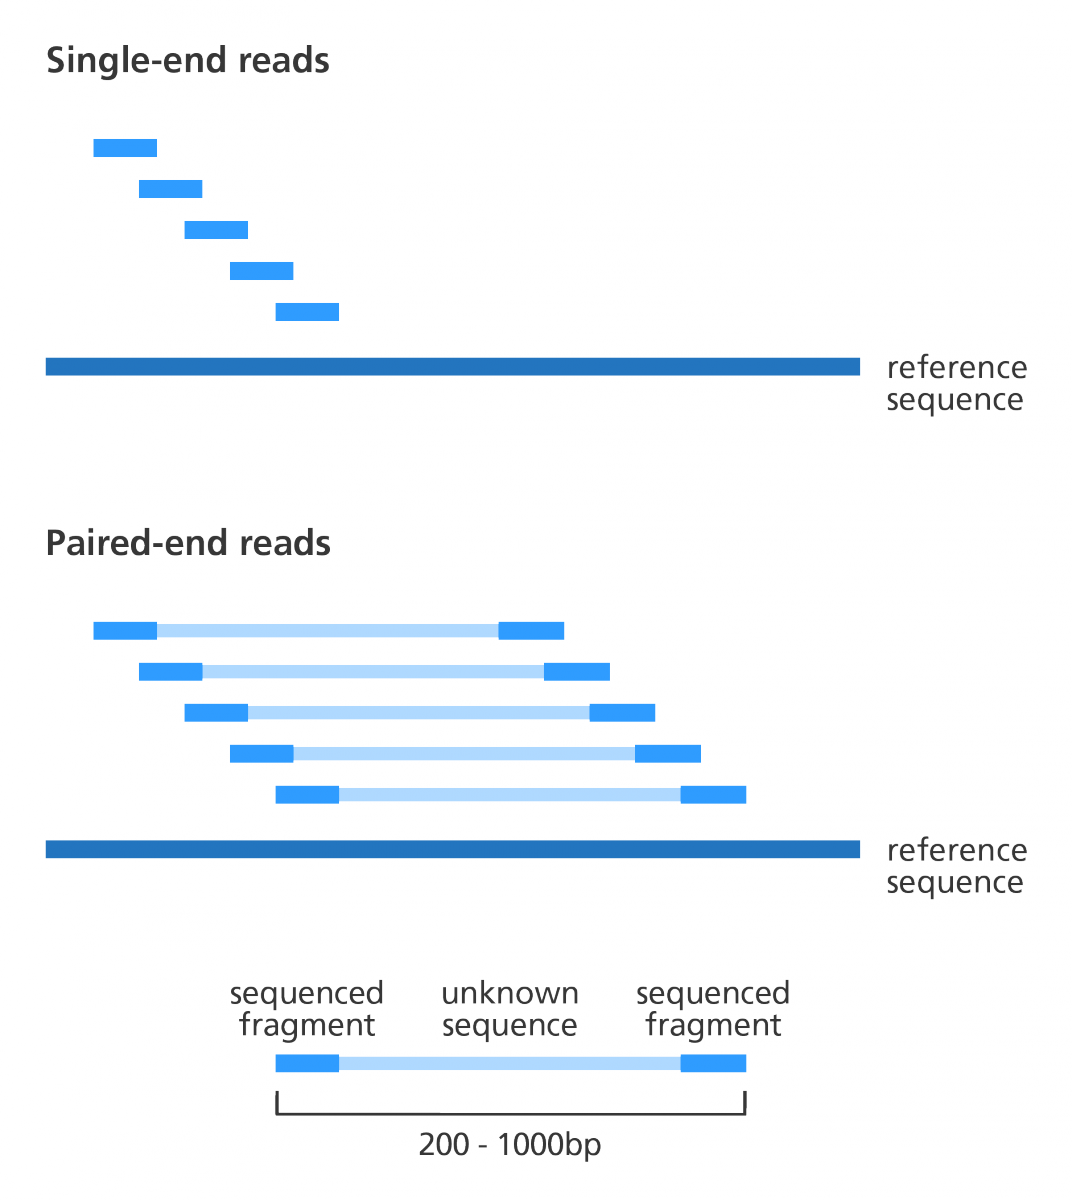
\includegraphics[height=10cm,width=10cm]{images/pairedendreads.png}
  \caption{Esempi di read single-end e paired-end}
  \label{fig:PairedEndReads}
\end{figure}